\documentclass[11pt,letterpaper]{article}
\usepackage{fullpage}
\usepackage[top=1.75cm, bottom=4cm, left=1.25cm, right=1.25cm]{geometry}
\usepackage{amsmath,amsthm,amsfonts,amssymb,amscd}
\usepackage{lastpage}
\usepackage{enumerate}
\usepackage{fancyhdr}
\usepackage{mathrsfs}
\usepackage{xcolor}
\usepackage{graphicx}
\usepackage{listings}
\usepackage{hyperref}
\usepackage{tcolorbox}
\usepackage{bbm}
\usepackage{cite}
\usepackage[numbers]{natbib}

% \usepackage[utf8]{inputenc}
% \usepackage{amsmath, amsfonts, mathrsfs}
% \usepackage{enumitem}
% \usepackage{wrapfig}
% \usepackage{hyperref}
% \usepackage{indentfirst}
% \usepackage{placeins}
% \usepackage{xcolor}
% \usepackage{comment}
% \usepackage{float}

\hypersetup{%
colorlinks=true,
urlcolor=blue,
citecolor=blue
}

\renewcommand\lstlistingname{Algorithm}
\renewcommand\lstlistlistingname{Algorithms}
\def\lstlistingautorefname{Alg.}

\lstdefinestyle{Python}{
  language        = Python,
  frame           = lines,
  basicstyle      = \footnotesize,
  keywordstyle    = \color{blue},
  stringstyle     = \color{green},
  commentstyle    = \color{red}\ttfamily
}

\setlength{\parindent}{0.0in}
\setlength{\parskip}{0.05in}

\newtcolorbox{cbox}[3][]
{
  colframe = #2!25,
  colback  = #2!10,
  coltitle = #2!20!black,
  title    = {#3},
  #1,
}

\newcommand\course{CS 674}
\newcommand\instructor{Dr. Wingate}
\newcommand\name{Jake Callahan, Taylor Paskett}

\pagestyle{fancyplain}
\headheight 32pt
\lhead{\name \\ \today}
\chead{\textbf{}}
\rhead{\course \\ \instructor}
\lfoot{}
\cfoot{}
\rfoot{\small\thepage}
\headsep 1.5em

\title{Gaussian Process Guided Neural Networks: An Exploration}
\author{\name}

\begin{document}

\maketitle

\section{Introduction}
  A major problem facing neural networks today is the size of their required training set. Neural networks need a large amount of data to train an accurate model. Further, neural networks can only learn relationships that exist in these data, and aren't well-suited to ingesting and learning from prior knowledge about the data.

  Conversely, many Bayesian inference- based statistical methods are well-suited for training with smaller amounts of data and rely on imposed prior knowledge. However, they suffer from infeasibility at large scales and lack versatility across problem types.

  We propose a network architecture that combines the strengths of these models and mitigates their weaknesses.
  Inspired by physics-guided neural networks (PGNN), which rely on physical models to guide the training of the neural network \cite{PGNN}, we create a similar network that uses a Gaussian process to guide the training of a conventional neural network.

  In this paper, we find that on a face-pose detection problem, the Gaussian Process Guided Neural Network (GPGNN) achieves similar results to the current state-of-the-art \cite{whenet}, although more analysis is needed.

\section{Regular model vs. GPGNN}
A Gaussian Process-Guided Neural Network (GPGNN) can be used with any neural network architecture in a supervised learning task.
Let $ N(\cdot) $ represent the neural network and $ GP(\cdot) $ represent the trained Gaussian process.
Then, the only change to the training is that a regularized loss term is added to the original loss.
If the original loss is given by $ \mathscr{L}(y, \hat{y}) $ (for labels $ y $ and predictions $ \hat{y} $), then the GPGNN loss is given by \begin{align*}
    \mathscr{L}(y, \hat{y}) + \lambda P_{GP}(\hat{y} | y),
\end{align*}
for regularization constant $ \lambda \in \mathbb{R} $ and where $ P_{GP}(\hat{y} | y) $ represents a negative relative log likelihood of $ \hat{y} $ compared to $y$.
This likelihood is determined by the Gaussian process, and because of the way that Gaussian processes are defined, it's fairly easy to compute.
Specifically, letting $ \phi_X(\cdot) $ be the probability density function of the multivariate Gaussian distribution determined by the Gaussian process at input $ X $, we have \begin{align*}
     P_{GP}(\hat{y} | y) &= -\log \left( \frac{\phi_X(\hat{y})}{\phi_X(y)} \right) \\
     &= \log(\phi_X(y)) - \log(\phi_X(\hat{y})).
\end{align*}

At this point, it is prudent to ask what the Gaussian process gives that we can't already get from the data.
From an information-theoretic perspective, we can't gain "more" information by fitting a GP model to the data.
However, we may be putting the information in a form that's much easier to consume.

We know that Gaussian process regressors are kernel methods that fit a multivariate Gaussian distributions to any finite collection of input data points.
Near clusters of known data points, the GP will give a Gaussian with a small covariance, while areas with less data will typically have a much larger variance.
This means that the neural network will be more restricted in high data areas and less restricted in low data areas.
Additionally, the GP may help smooth the neural network's output.
If an appropriately smooth kernel is chosen for the GP, then the neural network's output will be regularized to more closely follow the smooth GP.

In general, we believe that GPGNNs will be most helpful in situations where there is less data than typically needed for a neural network, or in situations where we have informative prior beliefs about the data's distribution that we can encapsulate in the GP.

\section{Data}
  We apply our GPGNN model to a common problem: facial pose detection. Specifically, we use the 300W-LP dataset \cite{300wlp}. This dataset is composed of one input variable, a close-up facial image, and three outcome variables which define the facial pose: pitch, yaw, and roll. These pose parameters are given in degrees, and range from $-90^{\circ}$ to $90^{\circ}$. This dataset is widely used in face-pose estimation problems and as such is a natural choice for training the GPGNN.

\section{Architecture}
  \subsection{WHENet}
    We base our model architecture on Zhou and Gregson's WHENet model \cite{whenet}. This model is the current state-of-the art, and will be used as a baseline comparison for the success of our GPGNN. WHENet is an extension of the successful EfficientNet model developed by Tan and Le \cite{efn}. WHENet uses EfficientNet as its first layer. It then takes the EfficientNet outputs and applies two separate loss functions to each of the yaw, pitch, and roll.

    One loss function is a mean-squared error loss that measures the model's regression performance, and the other is a cross-entropy loss that measures how well the model would do if it were a classification problem. This cross-entropy loss is applied by first binning each of the yaw, pitch and roll into $60$ bins of $3$ degrees each, and then feeding these bins to the cross-entropy loss function. The total loss of the model is the sum across all loss terms. See Figure~\ref{fig:whenet_architecture} (courtesy of \cite{whenet}) for a visualization of this architecture.
    \begin{figure}[!htb]
    \centering
       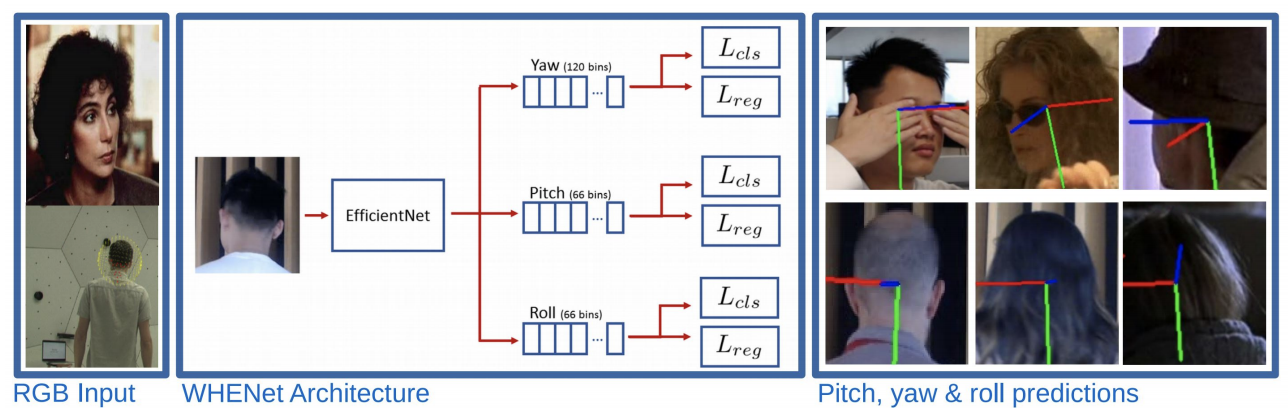
\includegraphics[width=0.65\linewidth]{./pics/whenet.png}
       \caption{Illustration of WHENet architecture}
       \label{fig:whenet_architecture}
    \end{figure}

  \subsection{GPGNN}
    Our GPGNN architecture is highly similar.
    We utilize the exact same WHENet architecture, simply adding the loss term $ \lambda P_{GP}(\hat{y}|y) $, with $ \lambda $ set to $ 1 $ (an arbitrary choice).
    In addition to selecting the neural network architecture, the parameters for the Gaussian process were chosen, and a GP was fit to the data.

    The Gaussian process used a scaled radial basis function kernel, \begin{align*}
        K(x,x') &= \alpha \exp( -\gamma \lVert x - x' \rVert^2 ).
    \end{align*}
    The parameters $ \alpha $ and $ \gamma $ were obtained via gradient descent based on the GP's marginal log-likelihood for the training data.

    Other considerations affected the training of the Gaussian process.
    In general, training a Gaussian process on a 1-dimensional data set of size $ N $ requires a training time with complexity of $ O(N^3) $.
    Gaussian processes are also expensive to train for high-dimensional datasets (partially due to the multivariate Gaussians that are computed).
    Because of this, training the GP on the 300W-LP dataset was too computationally expensive.
    So, we had to simplify in two ways:
    \begin{enumerate}[(1)]
       \item by reducing the dimensionality of the dataset;
       \item by reducing the number of points used to train the GP.
    \end{enumerate}
    To accomplish (1), we first performed principal component analysis on the dataset and used the first ten principal components for each image.
    To reduce the number of points used to train the GP (2), we performed k-means clustering on the PCA-transformed inputs, letting k=1000.
    Then, we trained the Gaussian process on the 1000 training data points nearest to each of the 1000 k-means centroids.


\section{Conclusion}
\subsection{Results of Experiment}
We found that after a few epochs, the WHENet and GPGNN had similar losses.
In Figure \ref{loss_fig}, we see that losses are comparable.
Due to time/computation constraints, we were not able to train for further epochs.
Training a larger number of epochs would give us more interesting and useful results here.

\begin{figure}[!htb]
\begin{center}
   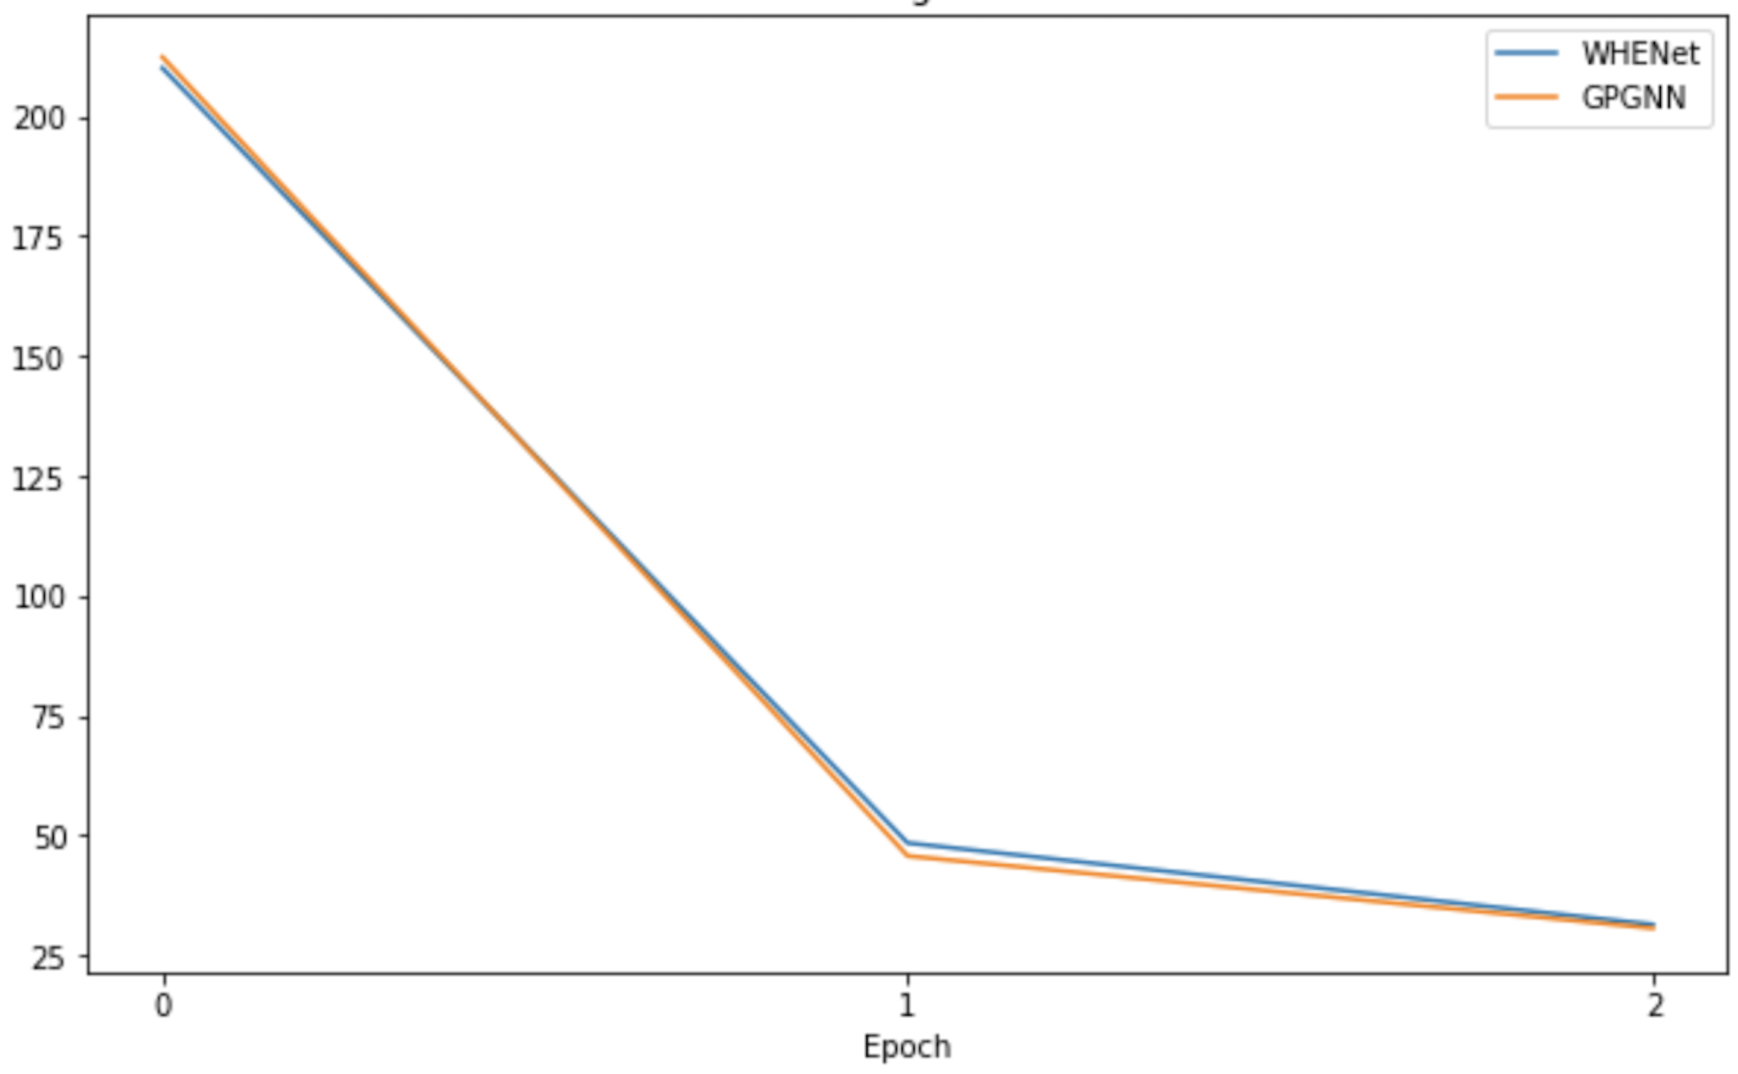
\includegraphics[width=0.55\linewidth]{./pics/training_loss.png}
   \caption{Comparing Similar Training Loss for Both Models}
   \label{loss_fig}
\end{center}
\end{figure}

We can also see the mean-squared error of the GPGNN predictions for pitch, yaw, and roll in Figure \ref{mse_fig}.

\begin{figure}[!htb]
\begin{center}
   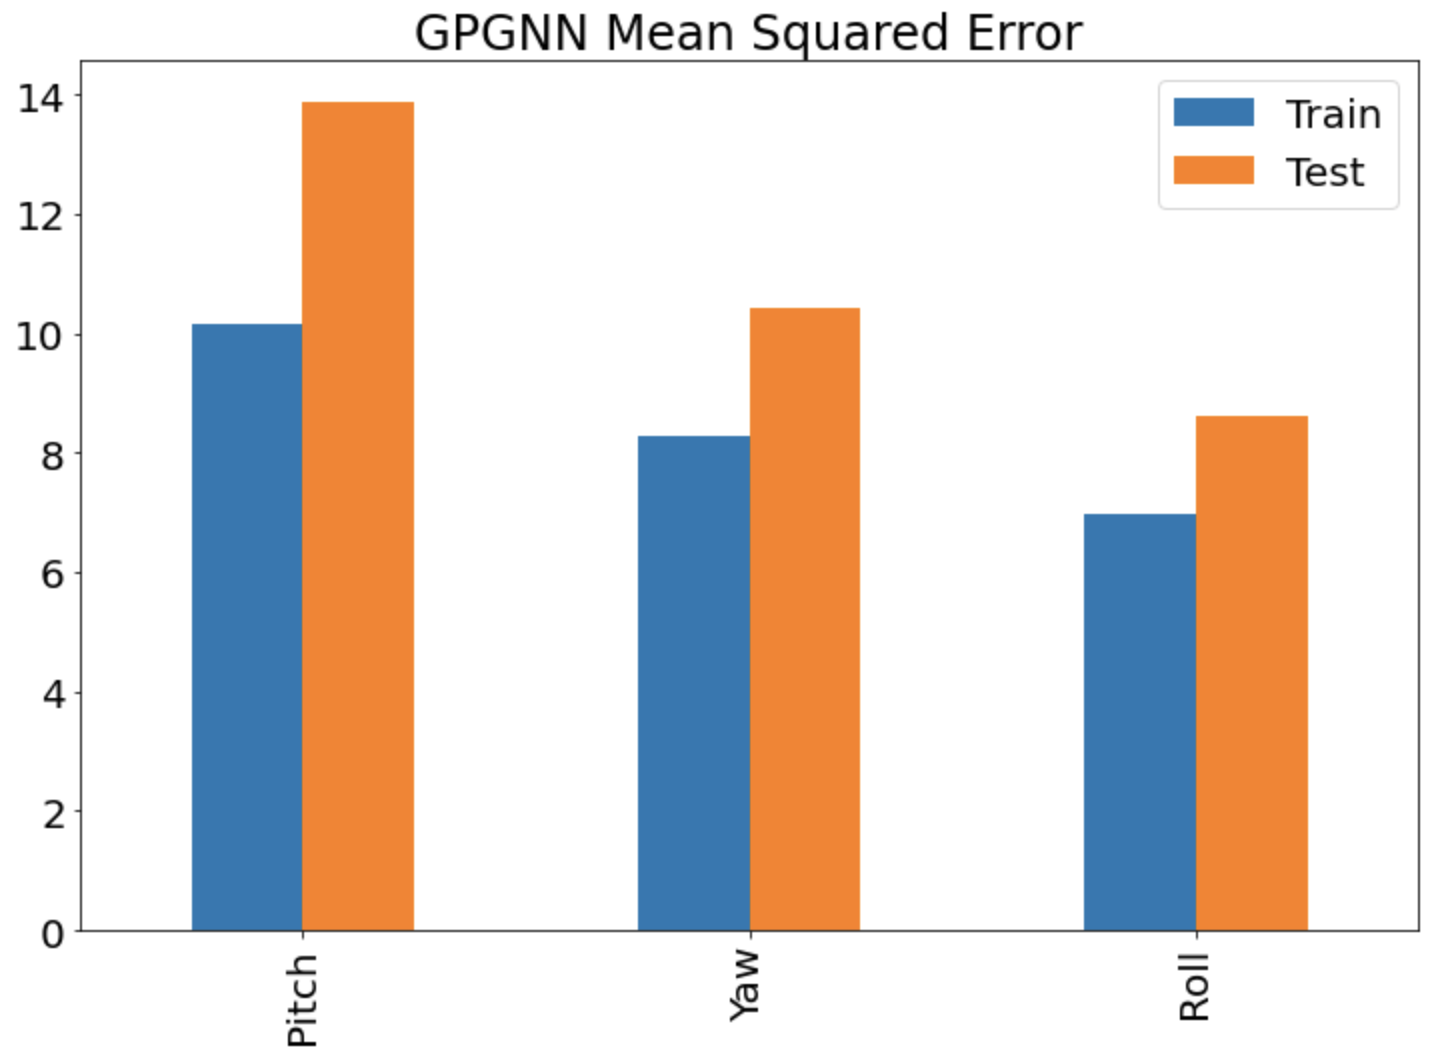
\includegraphics[width=0.55\linewidth]{./pics/mse_p_y_r.png}
   \caption{Comparing MSE on Train vs Test Data}
   \label{mse_fig}
\end{center}
\end{figure}

\subsection{Future Work}
In order to obtain more robust results or bring this idea to a publication level, we should do more extensive training.
First, training for a larger number of epochs would be useful.
Second, accuracy should be compared with GPGNNs that use other values for the regularization parameter $\lambda$.
As it currently stands, it could be that setting $ \lambda = 1 $ is not large enough to get much of an effect from the regularization term, explaining away our results.
Further cross-validation would help us understand the effect of the GPGNN and if it can achieve better results compared to the classic WHENet.
Third, training on a larger variety of regression tasks would be helpful.
Finally, it would be very interesting to train a GPGNN on a very sparse dataset.
Since standard neural networks rely on large training data sets, while Gaussian processes are well suited to smaller amounts of data, attempting a small-training-data task could give us further insight on the efficacy of GPGNNs.

Our work represents a proof of concept of a GPGNN.
It suggests that GPGNNs may be worth studying/building, but further analysis is needed to determine how useful they really are.


\bibliography{references.bib}{}
\bibliographystyle{plainnat}

\end{document}
